% !TEX TS-program = LuaLaTeX-shell

\documentclass[convert,tikz,border=5pt]{standalone}
\usepackage{tikz}
\usetikzlibrary{positioning,shapes.multipart,chains,calc}
\tikzset{my node/.style={on chain,join={by -stealth,very thick},draw,thick,font=\sffamily\strut, align=center,text width=3cm,minimum height=2cm,rounded corners,fill=#1}}
\begin{document}
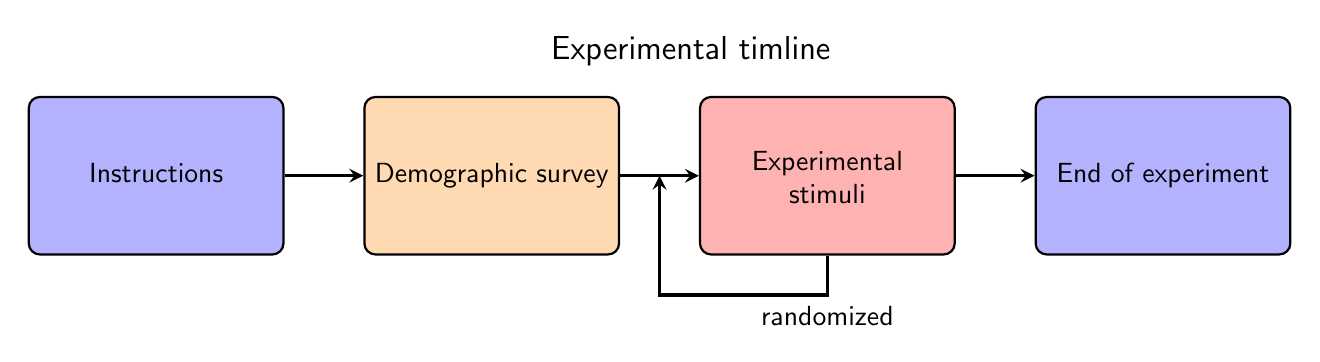
\begin{tikzpicture}[start chain]
\node[my node=blue!30] (instructions) {Instructions};
\node[my node=orange!30] (demographics) {Demographic survey};
\node[my node=red!30] (stimuli) {Experimental\\ stimuli};
\node[my node=blue!30] (end) {End of experiment};
\node[font=\sffamily\large,above right= .25cm and -1cm of demographics] {Experimental timline};
\draw[-stealth,very thick]
	(stimuli.south) --++ (0cm,-.5cm) -| node [below] {\sffamily randomized} ++(0cm,0cm) -| ($(stimuli.west) - (.5cm,0cm)$);
\end{tikzpicture}
\end{document}